\documentclass[12pt]{article}

%\usepackage{amsthm}%
\usepackage{amsmath}
\usepackage{amssymb}
\usepackage{amsfonts}
\usepackage[margin=0.75in]{geometry}
\usepackage{enumerate}
\usepackage{verbatim}
\usepackage{graphicx}
\usepackage{hyperref}
\usepackage{url}
\usepackage{times}
\usepackage[]{algorithm2e}
\usepackage[T1]{fontenc}
\newenvironment{proof}{\noindent{\bf Proof:} \hspace*{1mm}}{
        \hspace*{\fill} $\Box$ }
\newenvironment{proof_of}[1]{\noindent {\bf Proof of #1:}
        \hspace*{1mm}}{\hspace*{\fill} $\Box$ }
\newenvironment{proof_claim}{\begin{quotation} \noindent}{
        \hspace*{\fill} $\diamond$ \end{quotation}}

\newtheorem{thm}{Theorem}
\newtheorem{lemma}[thm]{Lemma}

\newcommand{\mbf}{\mathbf}
\newcommand{\mrm}{\mathrm}

\newcommand\abs[1]{\left|#1\right|}
\newcommand\given[1][]{\:#1\vert\:}
\newcommand{\legendre}[2]{\genfrac{(}{)}{}{}{#1}{#2}}
\newcommand{\port}{\texttt{port}}
\newcommand{\google}{\texttt{google}}
\newcommand{\starboard}{\texttt{starboard}}
\newcommand{\halibut}{\texttt{halibut}}

\setcounter{tocdepth}{1}
\newtheorem{theorem}{Theorem}
\pagenumbering{gobble}

\title{\vspace{-2cm}\textsc{EE16B} Final Project Writeup}
\author{%
        Christopher Branner-Augmon \\
          \texttt{ee16b-amb}
        \and
        Ahmed Husain \\
          \texttt{ee16b-amy}
        \and
        Peter Manohar \\
          \texttt{ee16b-aif}
        \and
        Pratyush Mishra \\
        \texttt{ee16b-aci}
        \and
        Amanda Tomlinson\\
        \texttt{ee16b-amu}
      }

\begin{document}
\maketitle
\section*{General}

The project gave us a better understanding of PCA and k-means. We also learned
how to implement control systems, and struggled with debugging the car.  We
encountered many issues with the car, coming from both the software and the
hardware. We discovered that changes in hardware could also result in changes
in software. This occurred when we switched the microphone circuit for speech
classification.

Sometimes the circuit schematic and values that were given to us did not work
well with our design. We found that the non-ideal conditions of reality can
force us to make minor changes to our theoretical circuit in order for the
system to work properly.  Our demo is available at
\url{https://www.youtube.com/watch?v=LVntcSF0hhY}.

\section*{PCA Classification}

We tried to pick words that had distinct lengths and distinct vowel sounds. We
initially tried only varying the length of the words, but found that
consistently fitting longer words in the short recording interval was
difficult.  So, to make make each word more distinct, we tried varying the
length and sound of vowels in our words. After some experimentation, we settled
on the words {\port}, {\halibut}, {\google}, and {\starboard}.

We chose {\port} because it was short, unlike all the other words.
\texttt{Starboard}, on the other hand, is the longest of our words. To vary the
vowels we used, we picked {\google} and {\halibut} to include a long ``o''
and short ``a'' sound.

We also pronounced each word in a very unusual manner to emphasize differences,
thus ensuring that the sampled waveforms would be clearly distinct.  This
helped improve the consistency of our classification. For example, when saying
the word \texttt{starboard}, we added an inflection (specifically, a rising ``ou''
sound) at the end of the word. Without this, our classification was not very
accurate.

We obtained distinct clusters for {\halibut}, {\google}, and {\starboard}
after projecting our data onto the principal components.  The data points
corresponding to {\port} were spread out, but did not interfere with the other
clusters. When we implemented the k-means classification on the
launchpad, we modified the algorithm slightly. Instead of using the same
threshold distance for all the clusters, we set different threshold distances
for each cluster. We did this because the cluster corresponding to {\port} was
significantly more spread out than the other clusters. Without this change we
were unable to classify {\port} correctly, since the data point was rarely
within the uniform minimum distance.

\section*{Controls}

The controls portion of the project was broken up into several steps. The first
step consisted of determining the open-loop model of the system. We
approximated the continuous-time system of each wheel using a discrete model,
with distance traveled and instantaneous velocity being state variables. Since
this system is discrete, we multiplied the velocity from the previous time step
by the time between samples and added this to the previous distance traveled.
This gave a good approximation of the actual distance traveled. With this
model, we could then describe our system as
\begin{align*}
  \begin{bmatrix}
    d[k+1] \\
    v[k+1]
  \end{bmatrix} &=
  \begin{bmatrix}
    1 & T_s \\
    0 & 1
  \end{bmatrix}
  \begin{bmatrix}
    d[k] \\
    v[k]
  \end{bmatrix} + B u[k]
\end{align*}
where $d$ is the distance
traveled so far, $v$ is the velocity, $T_s$ is the time between samples, and
$u$ is the control that we apply. For the second step, we had to choose the
eigenvalues of the closed loop matrix and then solve for feedback values that
would set those eigenvalues. Since our system has $2$ state variables and $u$
is a scalar input, $B$ had to be a column vector in order to satisfy
dimensionality requirements. The $B$ was determined by running the linear least
squares algorithm on each row of our system using the data collected from
running the dynamics\_data.ino file. The algorithm was used four times, since
it had to be done twice for each wheel. We employed a state feedback system
where our scalar input was the product of the feedback row vector $[F_1 \ F_2]$
and the state of the system. This yielded the following closed loop matrix
\begin{align*}
  A_{CL} &= \begin{bmatrix}
            1 + F_1 B_1 & T_s + F_1 B_2 \\
            F_1 B_2 & 1 + F_2 B_2
          \end{bmatrix}
\end{align*}

with the corresponding
characteristic polynomial \begin{flalign*} \lambda^2 + \lambda(-2 - F_1 B_1 -
F_2 B_2) + F_2 B_2 + F_1 B_1 - F_1 B_2 T_s + 1 = (\lambda -
\lambda_{d1})(\lambda - \lambda_{d2}) \end{flalign*} \indent We wrote down a
system of equations and solved for the feedback values in terms of the desired
eigenvalues. The eigenvalues were chosen to give a reasonable convergence time
while also ameliorating any oscillatory behavior. We ended up choosing
$\lambda_{d1} = \lambda_{d2} = 0.9$. For the final step we implemented
turning. To turn in a given direction, the wheel on that side needs to be
slower than the wheel on hte other side. Implementation was easy as we simply
changed the desired velocity of that wheel to a fraction of that of the other
wheel. We settled on a value of $0.045$ for the slower wheel, and $0.06$ for
the faster wheel.

\section*{Circuit}

\begin{figure}[htbp]
  \centering
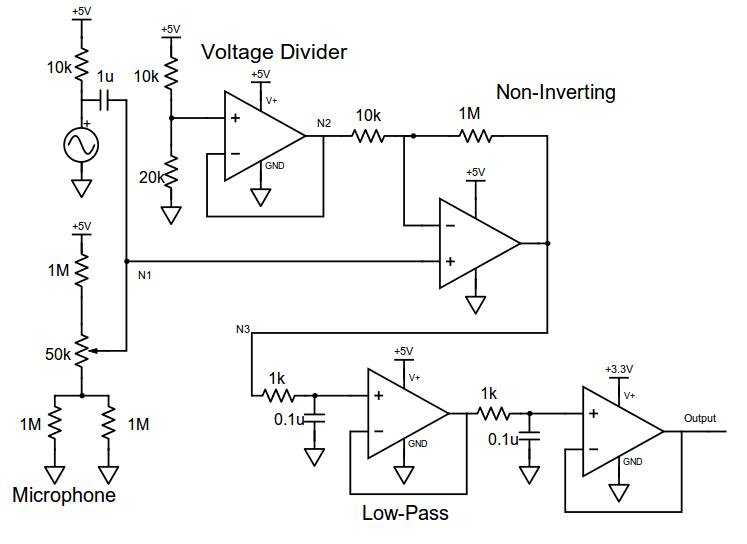
\includegraphics[width=350pt]{schematic.jpeg}
\caption{Circuit schematic.}
\label{fig:schematic}
\end{figure}


Our final schematic is seen in Figure~\ref{fig:schematic}.
The circuit has 3 main parts: the microphone circuit, a non-inverting
amplifier, and a second order low pass filter.

The microphone circuit was given from the specification, although we had to
make some slight changes. The potentiometer could not be tuned to the correct
value with the specification values, so we had to add an extra resistance to
ground. This allowed us to get our microphone signal centered at 1.6V. We
measured the output of our microphone using a pure tone as the input from a
distance of about $10$ cm, getting a reading of $\pm 50$ mV. In the actual
circuit we planned on getting a signal that was \\ $\pm$ 5mV since we would be
farther away. Therefore, at node $N_1$ in the circuit we anticipated a $\pm$
5mV signal, centered at $1.6$ V.

The next stage of the circuit was the amplification. Since the signal had a
small amplitude, we needed a very large amplification. We originally planned
for a gain of $300$, but that turned out to be too small so we used an
amplifier with a gain of $10^{5}$. Instead of referencing ground for this
amplifier, we referenced a virtual ground at node $N_2$. The $1.6$V virtual
ground kept the signal centered so it didn't rail.  After being amplified, at
node $N_3$ we expected a signal that was $\pm 1.6$ V, centered at $1.6$ V.

Then this signal was passed through 2 low pass filters, which filtered out
frequencies larger than 1.5kHz. Finally, the signal was passed through a final
buffer that had rails at $0$ V and $3.3$ V, to ensure that we wouldn't send in
too high of a voltage into our MSP.

Overall, the circuit was challenging and fun to design and implement. We ran
into a lot of issues that were rewarding to solve. Debugging a circuit can be
really tricky!
\end{document}
